\documentclass[12pt,a4paper,dvipsnames,usenames]{beamer}
%\documentclass[12pt,a4paper,dvipsnames,usenames,handout]{beamer}
% \usepackage{droid}
%\usepackage{lmodern}
%\usepackage{robotomono}
%\usepackage{lobstertwo}
\usepackage{url}
\usepackage{xcolor}
\usepackage{amsmath,varwidth,slashed}
\usepackage[utf8]{inputenc}
\usepackage[T1]{fontenc}
\usepackage{tikz,tikz-uml,xparse}
\usepackage[normalem]{ulem}
\usepackage{transparent}
\usepackage{appendixnumberbeamer}

% -------------------------- %
% Standard LaTeX definitions %
% -------------------------- %

\DeclareGraphicsExtensions{.pdf}
\renewcommand\textbullet{\ensuremath{\bullet}}

% ----------------------------------- %
% Various tikz styles and definitions %
% ----------------------------------- %

\usetikzlibrary{calc,intersections,positioning,matrix,chains,scopes}
\usetikzlibrary{decorations.pathmorphing,decorations.pathreplacing,shapes}
\newcommand{\tikzmark}[1]{\tikz[overlay,remember picture] \node (#1) {};}

\tikzumlset{fill class=RoyalBlue!20}

\tikzstyle{startnode} = [circle, draw, fill=Bittersweet!20, minimum size=10pt, inner sep = 0]
\tikzstyle{stopnode} = [startnode]
\tikzstyle{process} = [rectangle, minimum width=2cm, minimum height=.7cm, text centered, draw, fill=OliveGreen!20, align=center, font=\scriptsize]
\tikzstyle{dangerprocess} = [process, fill=BrickRed!20, draw=BrickRed, thick]
\tikzstyle{flowarrow} = [->, >=stealth, thick]

% ---------------------------------- %
% My default listings C++ code style %
% ---------------------------------- %

\lstset{%
  language=C++, basicstyle=\scriptsize\ttfamily, 
  keywordstyle=\color{OliveGreen}, identifierstyle=\color{RoyalBlue}, 
  commentstyle=\color{Brown}, stringstyle=\color{Bittersweet}, showstringspaces=false,  
  breaklines=true, prebreak=\mbox{{\color{Bittersweet}\tiny\ $\hookleftarrow$}}, 
  postbreak=\mbox{{\color{Bittersweet}\tiny$\to$\ }}, tabsize=5,
  morekeywords={%
    MyClass,unique_ptr,shared_ptr,weak_ptr,auto_ptr,
    make_unique, make_shared, default_delete,
    dynamic_pointer_cast, const_pointer_cast,
    scoped_ptr,QSharedPointer,QScopedPointer,QWeakPointer,
    ftring, SmartPtr, Shape, Circle, ShapeFactory, CircleFactory,
    Derived, Base
  }
}

\def\inline{\lstinline[basicstyle=\ttfamily\normalsize]}

% ---------------------------------------------------------------------------------------------------- %
% Various command for inline code instead of lstinline so that I don't have to update the keyword list %
% ---------------------------------------------------------------------------------------------------- %

\newcommand{\object}[1]{{\ttfamily \color{OliveGreen}#1}}
\newcommand{\function}[1]{{\ttfamily \color{RoyalBlue}#1}}
\newcommand{\std}[1]{{\ttfamily {\color{RoyalBlue} std::}{\color{OliveGreen}#1}}}
\newcommand{\boost}[1]{{\ttfamily {\color{RoyalBlue} boost::}{\color{OliveGreen}#1}}}

\newcommand{\uniqueptr}{\std{unique\_ptr}}
\newcommand{\sharedptr}{\std{shared\_ptr}}
\newcommand{\weakptr}{\std{weak\_ptr}}
\newcommand{\autoptr}{\std{auto\_ptr}}

% The base16 colour scheme?
\definecolor{sbase03}{HTML}{002B36}
\definecolor{sbase02}{HTML}{073642}
\definecolor{sbase01}{HTML}{586E75}
\definecolor{sbase00}{HTML}{657B83}
\definecolor{sbase0}{HTML}{839496}
\definecolor{sbase1}{HTML}{93A1A1}
\definecolor{sbase2}{HTML}{EEE8D5}
\definecolor{sbase3}{HTML}{FDF6E3}
\definecolor{syellow}{HTML}{B58900}
\definecolor{sorange}{HTML}{CB4B16}
\definecolor{sred}{HTML}{DC322F}
\definecolor{smagenta}{HTML}{D33682}
\definecolor{sviolet}{HTML}{6C71C4}
\definecolor{sblue}{HTML}{268BD2}
\definecolor{scyan}{HTML}{2AA198}
\definecolor{sgreen}{HTML}{859900}

\definecolor{Tropiteal}{RGB}{0,168,198}
\definecolor{TealDrop}{RGB}{64,192,203}
\definecolor{WhiteTrash}{RGB}{249,242,231}
\definecolor{AtomicBikini}{RGB}{174,226,57}
\definecolor{FeebleWeek}{RGB}{143,190,0}
\definecolor{ICantExpress}{RGB}{28,20,13}
\definecolor{Marty}{RGB}{250,42,0}

\colorlet{ColourBase}{Tropiteal}
\colorlet{ColourHl1}{Marty}
\colorlet{ColourHl2}{FeebleWeek}
\colorlet{ColourHl3}{TealDrop}
\colorlet{ColourDark}{ICantExpress}
\colorlet{ColourDark2}{Tropiteal}


\usetheme{metropolis}

\setbeamercolor{alerted text}{%
  fg=bazelGreen
}

\setbeamercolor{example text}{%
  fg=mLightBrown
}

\setbeamercolor{frametitle}{%
  use=normal text,
  fg=normal text.bg,
  bg=bazelGreen
}

\lstset{%
  basicstyle=\ttfamily\lst@ifdisplaystyle\fontsize{9pt}{9pt}\selectfont\fi,
  keywordstyle=\color{sgreen}, identifierstyle=\color{sblue}, 
  commentstyle=\color{sbase1}, stringstyle=\color{sorange},
  numberstyle=\color{sviolet}, showstringspaces=false,  
  breaklines=true,
  tabsize=5,
}

\lstalias[]{gnumake}[gnu]{make}

\newcommand{\dimtext}[2]%
{
  { \transparent{0.7}
  \begin{tikzpicture}[overlay, remember picture]
    \fill[white] ( #1 -| current page.north west) -- ++(0,.8em) -- ++(\paperwidth,0) -- (#2 -| current page.north east)
   -- ++(0,-.5em) -- ++(-\paperwidth,0) -- cycle;
  \end{tikzpicture}
  }
}

\newcommand{\specialcell}[2][c]{%
  \begin{tabular}
    [#1]{@{}c@{}}#2
  \end{tabular}
}

\newcommand{\tikzmark}[1]{\tikz[overlay,remember picture] \coordinate (#1);}

\newcommand{\qmat}{\ensuremath{Q_{\mathrm{uark}}}}
\newcommand{\mathfont}{\fontsize{10pt}{12pt}}
\newcommand{\minus}{\scalebox{0.75}[1.0]{$-$}}
\newcommand{\sectionframe}{%
  \addtocounter{framenumber}{-1}%
  \frame[plain]{\begin{center}\LARGE \color{beameralert} \insertsection\end{center}}}

\newcommand{\breakline}{%
  \begin{center} \begin{tikzpicture}
      \draw[beamerprimary] ({-0.5 * \textwidth},0) -- ({0.5 * \textwidth},0);
      \node[inner sep=0, minimum size=7pt, fill=white,circle] {};
      \node[inner sep=0, minimum size=4pt, draw=beamerprimary,circle] {};
      \node[inner sep=0, minimum size=1pt, fill=beamerprimary,circle] {};
  \end{tikzpicture} \end{center}
}


\setbeameroption{show notes}

\title{Analytic calculation of an effective lattice theory}
\author{Aleksandra R. Glesaaen}
\institute{
\includegraphics[scale=0.08]{Figs/GU-Logo-blau-CMYK.pdf}}
\date{Palaver July 06th 2015}

\begin{document}

\setlength{\abovedisplayskip}{0pt}
\setlength{\belowdisplayskip}{0pt}

\begin{frame}[plain]
  \titlepage
\end{frame}

\setcounter{framenumber}{0}

\begin{frame}
  \frametitle{Our Group}

  \begin{itemize}
    \setlength\itemsep{2em}
    \item Me: Started August 2013
    \item Group leader: Owe Philipsen
    \item Collaborator: Mathias Neuman
  \end{itemize}

\end{frame}

\begin{frame}
  \tableofcontents
\end{frame}

\section{Introduction}

\sectionframe

\begin{frame}
  \frametitle{The QCD Phase Diagram}

  {\centering%
    \only<1|handout:1>{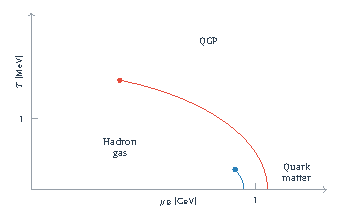
\includegraphics[scale=1.5]{Figs/phasediag.pdf}}%
    \only<2|handout:2>{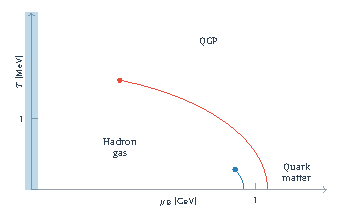
\includegraphics[scale=1.5]{Figs/phasediag2.pdf}}%
    \only<3|handout:3>{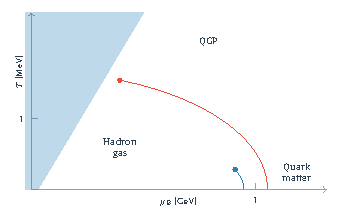
\includegraphics[scale=1.5]{Figs/phasediag3.pdf}}%
    \only<4|handout:4>{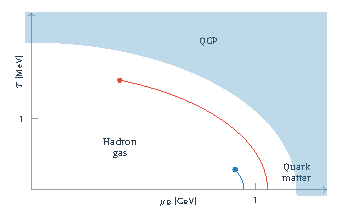
\includegraphics[scale=1.5]{Figs/phasediag4.pdf}}%
    \only<5|handout:5>{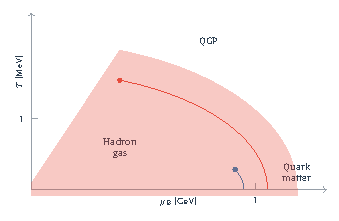
\includegraphics[scale=1.5]{Figs/phasediag5.pdf}}%
    \par
  }

  \begin{overlayarea}{\textwidth}{3em}
  \only<1|handout:1>{
  \begin{itemize}
    \item Different approaches can access different regions
  \end{itemize}}
  \only<2|handout:2>{
  \begin{itemize}
    \item Naive reach of Lattice QCD
  \end{itemize}}
  \only<3|handout:3>{
  \begin{itemize}
    \item Lattice QCD with additional methods \\ (analytic continuation, reweighting,...)
  \end{itemize}}
  \only<4|handout:4>{
  \begin{itemize}
    \item Perturbation theory of QCD
  \end{itemize}}
  \only<5|handout:5>{
  \begin{itemize}
    \item Region currently not accessible from first principles with traditional methods
  \end{itemize}}
  \end{overlayarea}

  \note<2>
  {
    Lattice QCD cannot natively deal with a finite baryon chemical potential because that turns the quark determinant into a
    complex quantity. On top of that we get important exponential cancellations coming from the "sign problem", which will be
    addressed later in this talk.
  }

  \note<3>
  {
    There are various techniques available to study finite density systems. With reweighting one uses the $\mu = 0$ system to
    evolve the Monte Carlo, then uses the actual $\mu \neq 0$ to measure observables. One can also measure the system at
    imaginary chemical potential and then use analytic continuation to extrapolate the results for $\mu^2 < 0$ to $\mu^2 > 0$.
  }

  \note<4>
  {
    Perturbation theory can of course only handle QCD at extreme temperatures and chemical potential, regions where the
    thermodynamic energy is large enough to have the QCD coupling run to values small enough for perturbation theory to be valid.
  }

  \note<5>
  {
    Most of the interesting phase structure is still in areas inaccessible to first principles theoretical approaches.
  }
\end{frame}

\begin{frame}
  \frametitle{Lattice QCD: Basics 1}

  \vfill

  Discretise space and time

  \vfill

  \begin{block}{Quarks}
      \[
       \mathcal{L}_F = \bar{\psi}(x) \big( i \gamma_{\mu} \partial^{\mu} + \gamma_{\mu} A^{\mu} \big) \psi(x) + m_q \bar{\psi}(x) \psi(x)
      \]
      \\[12pt]
      \[
        L_F \sim \sum_{\mu} \bar{\psi}(n) U_{\mu}(n) \psi(n+\mu) + m_q \bar{\psi}(n) \psi(n)
      \]
  \end{block}

  \begin{center}
  \begin{tikzpicture}
    \foreach \x in {1,...,6} {
      \foreach \y in {1,2} {
        \draw[LightUIBase!50!white] (\x,\y,0.7) -- (\x,\y,2.3);
      }
    }
    \foreach \x in {1,...,6} {
      \foreach \z in {1,2} {
        \draw[LightUIBase!50!white] (\x,0.7,\z) -- (\x,2.3,\z);
      }
    }
    \foreach \y in {1,2} {
      \foreach \z in {1,2} {
        \draw[LightUIBase!50!white] (0.7,\y,\z) -- (6.3,\y,\z);
      }
    }
    %\foreach \x in {1,...,6} {
      %\foreach \y in {1,2} {
        %\foreach \z in {1,2} {
          %\node at (\x,\y,\z) [circle, fill=LightUIBase,inner sep=0, minimum size=3pt] {};
        %}
      %}
    %}

    \node[fermion,fill=LightUIBlue] at (1,2,1) {};
    \node[fermion,fill=LightUIBlue] at (3,1,1) {};

    \path[draw=beameralert,thick,->-=.7] (1,1,2) -- (1,1,1);
    \node[fermion,fill=LightUIBlue] at (1,1,1) {};
    \node[fermion,fill=LightUIBlue] at (1,1,2) {};

    \path[draw=beameralert,thick,->-=.55] (2,1,2) -- (2,2,2);
    \node[fermion,fill=LightUIBlue] at (2,1,2) {};
    \node[fermion,fill=LightUIBlue] at (2,2,2) {};

    \path[draw=beameralert,thick,->-=.55] (3,2,1) -- (4,2,1);
    \node[fermion,fill=LightUIBlue] at (3,2,1) {};
    \node[fermion,fill=LightUIBlue] at (4,2,1) {};

    \path[draw=beameralert,thick,->-=.55] (5,1,2) -- (4,1,2);
    \node[fermion,fill=LightUIBlue] at (5,1,2) {};
    \node[fermion,fill=LightUIBlue] at (4,1,2) {};

    \path[draw=beameralert,thick,->-=.7] (6,2,1) -- (6,2,2);
    \node[fermion,fill=LightUIBlue] at (6,2,1) {};
    \node[fermion,fill=LightUIBlue] at (6,2,2) {};

  \end{tikzpicture}
  \end{center}

  \begin{tikzpicture}[overlay, remember picture]
    \draw[->,>=stealth] ([shift={(-.3,1.2)}] current page.center) -- +(0,-.6) node[midway,scale=0.75,right=4pt] {$x \to a n$};
  \end{tikzpicture}

  \note
  {
    See that the $\psi(n)$ variables have a set position $n$, and are thus are associated with the different points
    on our lattice. The variables $U_{\mu}(n)$ have both a position $n$, and a direction $\mu$. It can therefore for example be
    associated with to points, or more conveniently with the link between the two points.

    \vspace{1em}

    This is what we mean when we say that in Lattice QCD the quarks live on the sites and the gluons on the links.

    \vspace{1em}

    The first term in the QCD Lagrangian thus is a sort of directional nearest neighbour interaction, 
    where the interaction link itself is a variable.
  }
\end{frame}

\begin{frame}
  \frametitle{Lattice QCD: Basics 2}

  \vfill

  Discretise space and time

  \vfill

  \begin{block}{Gluons}
      \[
       \mathcal{L}_G = \frac{1}{4} \tr F_{\mu\nu}(x) F^{\mu\nu}(x)
      \]
      \\[10pt]
      \[
        L_G \sim \beta\sum_{\mu,\nu} \tr U_{\mu}(n) U_{\nu}(n+\mu) U^{\dagger}_{\mu}(n+\nu) U^{\dagger}_{\nu}(n)
      \]
  \end{block}

  \begin{center}
    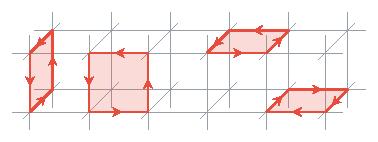
\includegraphics{Figs/gluonlagrange.pdf}
  \end{center}

  \begin{tikzpicture}[overlay, remember picture]
    \draw[->,>=stealth] ([shift={(-.3,1.2)}] current page.center) -- +(0,-.8) node[midway,scale=0.75,right=4pt] {$x \to a n$};
  \end{tikzpicture}

  \begin{tikzpicture}[overlay,remember picture]

    \coordinate (plaquette) at ([shift={(-1.2,1.2)}] current page.south);
    \node[scale=0.75] at ([shift={(5,-.5)}] plaquette) (label) {plaquette};

    \draw[<-,>=stealth] (plaquette).. controls +(0,-1.5) and +(-1,0) .. (label);
    \draw[->,>=stealth] (label).. controls +(0,1) and +(1,-1) .. ++(-1,3.7);
  \end{tikzpicture}

  \note
  {
    The link plaquette constites the smallest gauge invariant geometric quantity one can construct on the lattice using the group
    elements $U$. It is very similar to how one construct $F_{\mu\nu}$ in continuous Yang-Mills theory if one doesn't go the
    covariant derivative route.
  }

\end{frame}

\begin{frame}
  \frametitle{Lattice QCD: Basics 3}

  \begin{block}{Partition function}
    \begin{align*}
      \mathcal{Z} &= \int D U_{\mu} D \bar{\psi} D \psi \, \exp \Big\{ \minus \bar{\psi} \qmat \psi - S_{\mathrm{gluon}} \Big\} \\
      &= \int D U_{\mu} \det \qmat \exp \big\{ \minus S_{\mathrm{gluon}} \big\}
    \end{align*}
  \end{block}
  
  \vfill
  
  \noindent Measure observables by running a Monte Carlo simulation using

  \vfill

  \begin{block}{Monte Carlo weight}
  \begin{equation*}
    \det \qmat \exp \big\{ \minus S_{\mathrm{gluon}} \big\}
  \end{equation*}
  \end{block}

  \note
  {
    When doing lattice simulations, the integral over the fermion fields are done analytically which results in the determinant of
    the quark matrix $\qmat$. There are other ways of approaching this, but from a technical standpoint it is also convenient to
    get rid of the Grassmann-variables, as they are hard to deal with numerically. The remaining integral over the fields
    $U_{\mu}$ is a strongly coupled, highly dimensional integral that is almost impossible to solve in practice. Therefore we
    rather use the measure in the integral as a Monte Carlo weight, and can use a Monte Carlo simulation algorithm to evolve the
    system in a way that minimises the action, measuring observables along the way.

    \vspace{1em}

    One does thus not calculate $\mathcal{Z}$ in Lattice QCD, but one calculates observables: 
    $\langle O \rangle = \displaystyle\frac{1}{\mathcal{Z}} \displaystyle\int \mathrm{D} U \, O(U) e^{\minus S}$
  }

\end{frame}

\begin{frame}
  \frametitle{Lattice QCD: Challenges}
  \framesubtitle{Simulation cost}

  Counting the degrees of freedom of the system gives a staggering number

  \vspace{.5em}

  \[
    N = N_t \times N_x \times N_y \times N_z \times N_{\gamma} \times N_f \times N_c
  \]

  \vspace{1em}

  Every simulation point must evaluate $\det \qmat$, \\
  which is a (sparse) $N \times N$ matrix

  \note
  {
    Running Lattice simulations at large volumes and small quark masses gets extremely expensive, which is why 
    we need supercomputers and months of computation time to get the configurations. The quark determinant in particular
    is numerically demanding to calculate due to its sheer size, which is at least as slow as the best LU-decomposition
    algorithm.

    If one wants lighter quarks, the amount of statistics needed to suppress the statistical errors become very large,
    and the computation times sky-rocket.
  }

\end{frame}

\begin{frame}
  \frametitle{Lattice QCD: Challenges}
  \framesubtitle{The sign problem 1}

  Lattice QCD relies on Monte Carlo integration for the integral over link variables

  \vspace{2em}

  \begin{block}{}
    \begin{equation*}
      Z = \int D U_{\mu} \det \qmat e^{\minus S_{\mathrm{gluon}}}
    \end{equation*}
  \end{block}

  \vspace{1em}

  It only makes sense to use {\mathfont $\det \qmat e^{\minus S_{\mathrm{gluon}}}$} as a \\
  Monte Carlo weight if it is real

  \note
  {
    The second important limitation we want to look at for Lattice QCD is the so called "sign problem". It relates to the fact
    that without a baryon chemical potential, the fermion determinant is strictly real for all values of the gauge fields $U$. If
    we introduce a baryon chemical potential term to our lagrangian, $\mu\bar{\psi} \gamma_0 \psi$, the quark matrix gets complex
    values. Integrated over all configurations of $U$, the end result is of course real, so the imaginary components cancel out in
    the end. However, we sample the determinant with a Monte Carlo simulation, and thus getting these exact calculations is
    impossible. Also, it makes no sense to use $\det \qmat$ as a probability if it is complex.
  }
\end{frame}

\begin{frame}
  \frametitle{Lattice QCD: Challenges}
  \framesubtitle{The sign problem 2}

  %\only<1|handout:1>{

  The link integral also suffer from exponensial cancellations

  \vspace{1em}

  Example
  %}

  \begin{columns}
    \column{.3\textwidth}
    {\fontsize{10pt}{12pt} \raggedleft 
      \(
        f(x) = e^{\minus x^2 + i\theta x}
      \) \par
    }
    \column{.7\textwidth}
    \begin{center}
      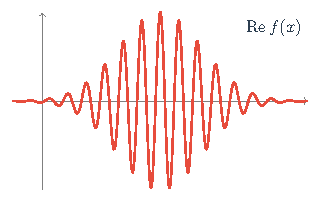
\includegraphics{Figs/plot.pdf}
      %\only<1|handout:1>{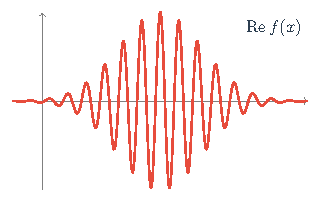
\includegraphics{Figs/plot.pdf}}
      %\only<2|handout:2>{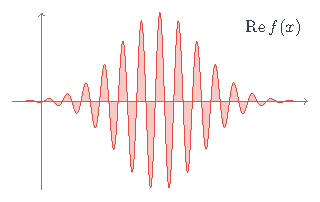
\includegraphics{Figs/plot2.pdf}}
      %\only<3|handout:3>{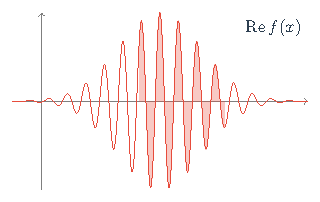
\includegraphics{Figs/plot3.pdf}}
    \end{center}
  \end{columns}

  %\only<2-|handout:2,3>{\breakline}

  %\begin{onlyenv}<2|handout:2>
    %\begin{minipage}[c][1cm]{\textwidth}
    %\mathfont
    %\[
      %\int_{-\infty}^{\infty} \mathrm{d} x \, f(x) = \sqrt{\pi} e^{\minus\frac{\theta^2}{4}}
    %\]
    %\end{minipage}
  %\end{onlyenv}

  %\begin{onlyenv}<3|handout:3>
    %\begin{minipage}[c][1cm]{\textwidth}
      %$\displaystyle\int_a^b \hskip-2pt \mathrm{d} x \, f(x)$ strongly depend on $\theta$ and $[a,b]$
    %\end{minipage}
  %\end{onlyenv}

  \note
  {
    To demonstrate this point we have a classical example. Consider the function on the slide, which is an exponential with a
    complex phase. If we carry out the full integral, the imaginary parts of $f$ all cancel out, and we are left with a real
    number. However the final result is exponentially suppressed by the frequency of the complex phase. On top of that, if we
    choose the boundaries in an unfortunate way, the final result will strongly depend on the boundaries. This is an issue as we
    in Lattice QCD do not have a strict control over our "boundaries" because the configurations are generated randomly.
  }

\end{frame}

\section{The Effective Theory}

\sectionframe

\begin{frame}
  \frametitle{The Effective Lattice Theory}

  \begin{alertblock}{Our goal}
    \begin{itemize}
      \item \color{LightUIBase} Integrate out all spatial gauge links
    \end{itemize}
    \begin{align*}
      \mathcal{Z} &= \int D U_{\mu} \exp\big\{ \minus S_{\mathrm{action}} \big\} \\
      &= \int D U_0 \exp\big\{ \minus S_{\mathrm{effective \: action}} \big\}
    \end{align*}
  \end{alertblock}

  \note
  {
    We create an effective action by carrying out some of the gauge link integrals by hand. Similar to how we got an effective
    action for the gluons by integrating out the fermions in the beginning, we get an effective action for the gauge links
    pointing in time direction by integrating out all the link pointing in spatial directions.

    \vspace{1em}

    The reason we pick out the time direction specifically is of course because the time direction plays a special role for
    Thermal Field Theories. One introduces temperature into a quantum field theory by compactifying the temporal direction,
    meaning introducing period boundary-conditions, under which the fermions and bosons transform in different ways.
  }

\end{frame}

\begin{frame}
  \frametitle{Strong Coupling Expansion}

  Expansion around $\beta = \scalebox{0.75}{$\displaystyle\frac{2 N_c}{g^2}$} = 0$

  \vspace{2em}

  \begin{block}{Recap}
    \[ L_G \sim \beta\sum_{\mu,\nu} \tr U_{\mu}(n) U_{\nu}(n+\mu) U^{\dagger}_{\mu}(n+\nu) U^{\dagger}_{\nu}(n) \]
  \end{block}

  \vspace{1em}

  This is an expansion in the number of plaquettes on the lattice

  \note
  {
    So the cost of putting one plaquette on the lattice is of the order $\beta$. If we take $\beta$ to be small, we thus order by
    order add one more plaquette to the lattice. The smallest non-zero contribution is gotten by adding 6 plaquettes formed in a
    cube, but that only contributes to vacuum physics, so we aren't interested in that.
  }

\end{frame}

\begin{frame}
  \frametitle{Hopping Parameter Expansion}

  One can rewrite the fermion matrix $\qmat$ as
  
  \vspace{2em}

  \begin{block}{}
    \[
      \det \qmat = \exp \bigg\{ - \sum_{n=1}^{\infty} \frac{1}{n} \kappa^n \tr H_{\mathrm{op}}^n \bigg\}
    \]
  \end{block}

  \vspace{1em}

  where $H_{\mathrm{op}}$ translates the quark one lattice spacing and \\ $\kappa \sim 1/m_q$

  \note
  {
    The $\tr H_{\mathrm{op}}^n$ makes the fermion translate $n$ lattice spacings. Because there is a trace, which also is a trace
    in space-time, the fermion has to hop in a loop. Because of the spin structure, a fermion cannot do any "backtracking".
    Meaning it cant hop forward then backward the same direction, simply because $(1 + \gamma_{\mu})(1 - \gamma_{\mu}) = 0$.
  }

\end{frame}

\begin{frame}
  \frametitle{The Effective Lattice Theory}
  \framesubtitle{Pure gluon contributions}

  \only<1-3|handout:1>{
  \begin{center}
    \only<1|handout:0>{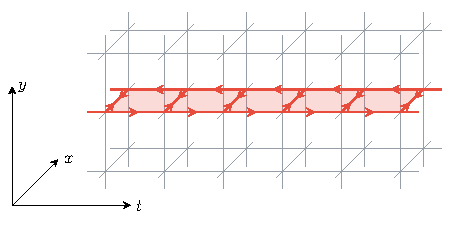
\includegraphics{Figs/puregauge1.pdf}}
    \only<2|handout:0>{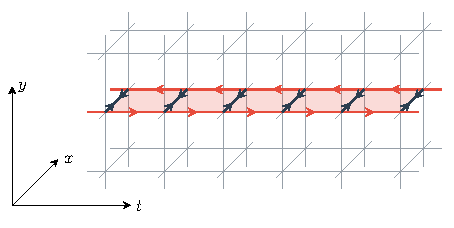
\includegraphics{Figs/puregauge2.pdf}}
    \only<3|handout:1>{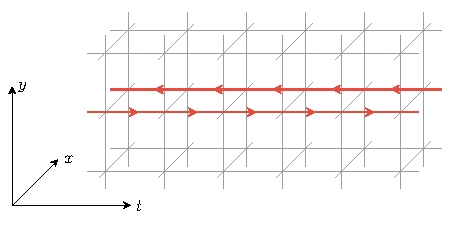
\includegraphics{Figs/puregauge3.pdf}}
  \end{center}
  }


  \only<1|handout:0>{
    Put a line of plaquettes in the time direction
  }
  \only<2|handout:0>{
    Integrate over all spatial gauge links
  }
  \only<3|handout:1>{
  What remains is an interaction between Polyakov Loops
  }

  \begin{onlyenv}<4|handout:2>

    \begin{block}{Effective Gluon Interactions}
      \begin{equation*}
        S_{\mathrm{eff \: gluon}} \sim \lambda \sum_{\langle x,y \rangle} L(x) L^*(y)
      \end{equation*}
    \end{block}

    \vspace{1em}

    \begin{center}
    \begin{tikzpicture}
      \draw[LightUIBase!50!white,use as bounding box] (-.3,-.3) grid[xstep=2] (6.3,2.3);
      \draw[thick,decorate, decoration={snake}, draw=LightUIBase] (2,1) -- (4,1)
        node[scale=0.75,midway,below=.2] {$\lambda$};
      \node[scale=2,fermion,fill=LightUIRed] at (4,1) (ell) {};
      \node[scale=0.75,above right=3pt of ell] {$L$};
      \node[scale=2,draw=LightUIRed, thick, circle, inner sep=0pt, minimum size=4pt] at (2,1) (elles) {};
      \node[scale=0.75,above left=3pt of elles] {$L^*$};

      \coordinate (coordcenter) at (-1,-1);
      \draw[->,>=stealth] (coordcenter) -- +(2,0) node[right,scale=0.75] {$x$};
      \draw[->,>=stealth] (coordcenter) -- +(0,2) node[right,scale=0.75] {$y$};
    \end{tikzpicture}
    \end{center}
     
    \vspace{1em}
  \end{onlyenv}

  \onslide<3|handout:1>{
  \begin{tikzpicture}[overlay, remember picture]
    \draw[<-,>=stealth] ([shift={(2.5,-.05)}] current page.center) .. controls +(.1,-.7) and +(-.3,0) .. +(2,-.4)
      node[scale=0.75,right] {$L$};
    \draw[<-,>=stealth] ([shift={(2.7,.5)}] current page.center) .. controls +(.1,.7) and +(-.3,0) .. +(2,+.4)
      node[scale=0.75,right] {$L^*$};
  \end{tikzpicture}
  }

  \note<3>
  {
    As mentioned earlier, we are only interested in quantities that contribute to the thermodynamic of the system. For our system,
    that means quantities which span the full temporal direction, and thus picks up a temperature dependent component in the
    infinite volume limit.

    For pure gauge action, in the strong coupling expansion, this means a plane of plaquettes spanning the full temporal
    direction, as shown in the figure. We then integrate out the spatial links present in this strip of plaquettes, and are left
    with the Polyakov loops.
  }

  \note<4>
  {
    The final result will thus be a nearest neighbour interaction between two Polyakov loops, or a continuos spin-system on a
    three dimensional lattice.
  }
\end{frame}

\begin{frame}
  \frametitle{The Effective Lattice Theory}
  \framesubtitle{Pure quark contributions}

  \only<1-3|handout:1>{
  \begin{center}
    \only<1|handout:0>{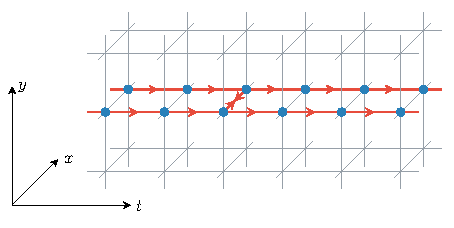
\includegraphics{Figs/purequark1.pdf}}
    \only<2|handout:0>{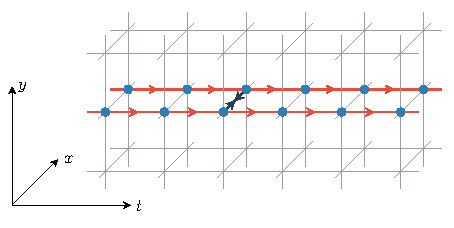
\includegraphics{Figs/purequark2.pdf}}
    \only<3|handout:1>{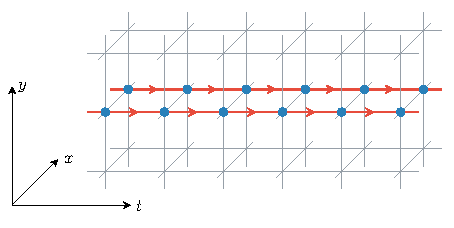
\includegraphics{Figs/purequark3.pdf}}
  \end{center}
  }

  \only<1-3|handout:1>{
  \begin{overlayarea}{\textwidth}{3em}
  \only<1|handout:0>{
    Can produce a closed quark loop with multiple temporal windings
  }
  \only<2|handout:0>{
    Once again integrate out spatial links
  }
  \only<3|handout:1>{
    Producing an interaction between the $W$ objects
  }
  \end{overlayarea}}

  \begin{onlyenv}<4|handout:2>

    \begin{block}{Effective Gluon Interactions}
      \[
        S_{\mathrm{eff \: quarks}} \sim h_2 \sum_{\langle x,y \rangle} W(x) W(y)
      \]
    \end{block}

    \vspace{1em}

    \begin{center}
    \begin{tikzpicture}
      \draw[LightUIBase!50!white,use as bounding box] (-.3,-.3) grid[xstep=2] (6.3,2.3);
      \draw[thick,decorate, decoration={snake}, draw=LightUIBase] (2,1) -- (4,1)
        node[scale=0.75,midway,below=.2] {$h_2$};
      \node[scale=2,draw=LightUIBlue, thick, circle, inner sep=0pt, minimum size=4pt] at (2,1) (w1) {};
      \node[scale=2,draw=LightUIBlue, thick, circle, inner sep=0pt, minimum size=4pt] at (4,1) (w2) {};
      \node[scale=0.75,above right=3pt of w2] {$W$};
      \node[scale=0.75,above left=3pt of w1] {$W$};

      \coordinate (coordcenter) at (-1,-1);
      \draw[->,>=stealth] (coordcenter) -- +(2,0) node[right,scale=0.75] {$x$};
      \draw[->,>=stealth] (coordcenter) -- +(0,2) node[right,scale=0.75] {$y$};
    \end{tikzpicture}
    \end{center}
     
    \vspace{1em}
  \end{onlyenv}

  \onslide<3|handout:1>{
  \begin{tikzpicture}[overlay, remember picture]
    \node[scale=0.75] at ([shift={(5,.55)}] current page.center) (wNode) {$W[L]$};
    \draw[<-,>=stealth] ([shift={(2.5,.2)}] current page.center) .. controls +(.1,-.7) and +(-.3,0) .. ([yshift=-1] wNode.west);
    \draw[<-,>=stealth] ([shift={(2.9,.8)}] current page.center) .. controls +(.1,.7) and +(-.3,0) .. ([yshift=1] wNode.west);
  \end{tikzpicture}
  }

  \note<3>
  {
    For the fermions we are in very much the same situation. We need a quantity that spans the temporal direction of the lattice.
    The simplest such object is of course a single quark line, exclusively jumping in the temporal direction, going around the
    lattice. This is the contribution from static quarks, and this is of course included.

    The next order term would be a quark that loops, jumps to a neighbouring site, loops, then jumps back, which is the term
    depicted in the figure. Here again we integrate out the spatial links, and are left with the interaction of two $W$-terms, the
    mathematical structure of which is not important for now.
  }

\end{frame}

\begin{frame}
  \frametitle{The Effective Lattice Theory}
  \framesubtitle{Final form}

  \begin{alertblock}{The Effective Action} \vspace{5pt}
    \[
      \mathcal{Z} = \int \prod_x \mathrm{d} L(x) \, \exp \big\{ \minus S_{\mathrm{eff \: action}} \big\}
    \]
    \[
      S_{\mathrm{eff \: action}} \sim \lambda \sum_{\langle x, y \rangle} L(x) L^*(y) + h_2\sum_{\langle x, y \rangle} W(x) W(y)
    \]
  \end{alertblock}

  \vspace{1em}

  Two options to proceed from here

  \begin{enumerate}
    \item Simulate the effective action
    \item \only<2>{\color{LightUIRed}}Analytically calculate it with a linked cluster expansion
  \end{enumerate}

  \note<2>
  {
    Since the effective action still is in the exponential, it is impossible to carry out the integrals analytically, but we have
    significantly reduced the complexity of the system. The fermion determinant is no more, and we have also decreased the number
    of free parameters by orders of magnitude.

    One way forward is to use the new action with a Monte Carlo simulation, which is what one of my colleage is doing. Another
    option would be to use a linked cluster expansion method to calculate the free energy from this analytically, and thus get
    expressions for baryon number density and other things analytically. This is the approach I have taken.
  }

\end{frame}

\begin{frame}[plain]
  \begin{tikzpicture}[overlay,remember picture]
    \node[anchor=north] at ([shift={(0,.3)}] current page.north)
    {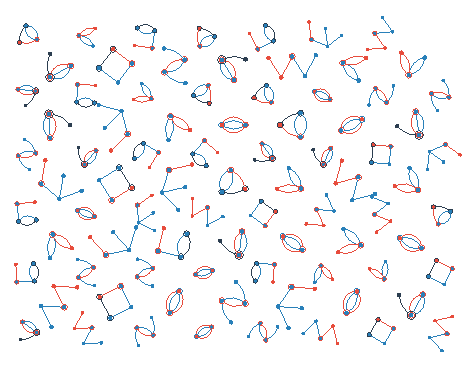
\includegraphics[scale=1.6]{Graphs/graphmatrix.pdf}};
  \end{tikzpicture}
  \note
  {
    Simply a fun slide to make fun at what I put myself through to get the result analytically rather than numerically.
  }
\end{frame}

\section{Results}

\sectionframe

\begin{frame}
  \frametitle{Comparison with Simulation}

  {\centering%
    \only<1|handout:0>{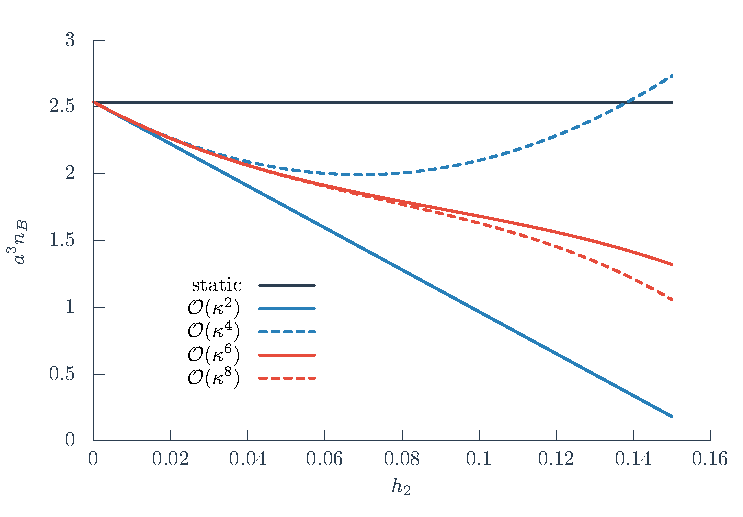
\includegraphics[width=\textwidth]{Plots/nucleon_number.pdf}}%
    \only<2|handout:0>{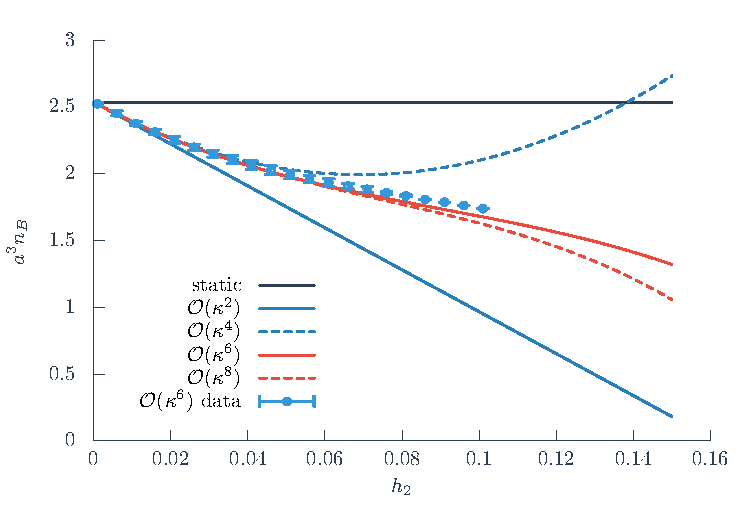
\includegraphics[width=\textwidth]{Plots/nucleon_number_w_k6.pdf}}%
    \only<3|handout:1>{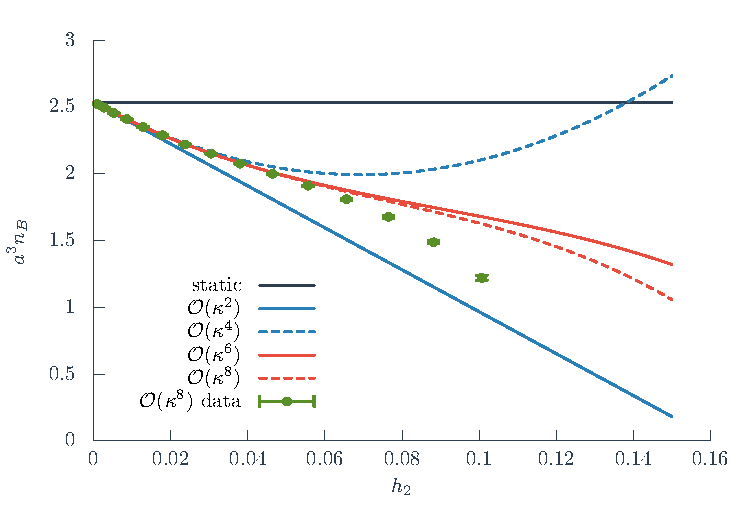
\includegraphics[width=\textwidth]{Plots/nucleon_number_w_k8.pdf}}%
  \par}

  \begin{tikzpicture}[overlay,remember picture]
    \draw[->,>=stealth] ([shift={(2.5,1.15)}] current page.south) -- +(2,0)
      node[midway,below,scale=0.65] {$m_q \to 0$};
  \end{tikzpicture}

  \note<3>
  {
    First of all see that it seems like the effective theory converges quite nicely as one systematically increases the order of
    $h_2$. When compared with simulations it also looks quite OK, however the $\kappa^8$ result seem to fail, but that might also be
    caused by the $\kappa^6$ just being a lucky hit. It should be noted that the error bars are actually way off, and do not
    represent the accuracy of the actual data, but are error bars for a certain element of the statistics carried out by the Monte
    Carlo algorithm. We are also having some numerical issues with simulating the effective theory at high order, so that might
    also disturb the results somewhat.
  }
\end{frame}

\begin{frame}
  \frametitle{Equation of State}

  \only<1>{
  {\centering
    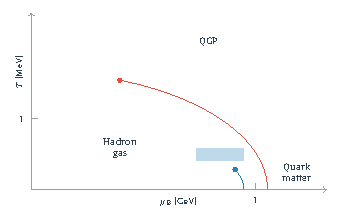
\includegraphics[width=\textwidth]{Figs/phasediag6.pdf}%
  \par}

  \begin{tikzpicture}[overlay,remember picture]
    \draw[<-,>=stealth] ([shift={(1.5,-1.2)}] current page.center) .. controls +(0,1) and +(-.5,-.5) ..  ++(1,2)
    node[right,scale=.75,align=center] {we are \\ $\approx$ here};
  \end{tikzpicture}
  }

  \only<2>{
  {\centering%
    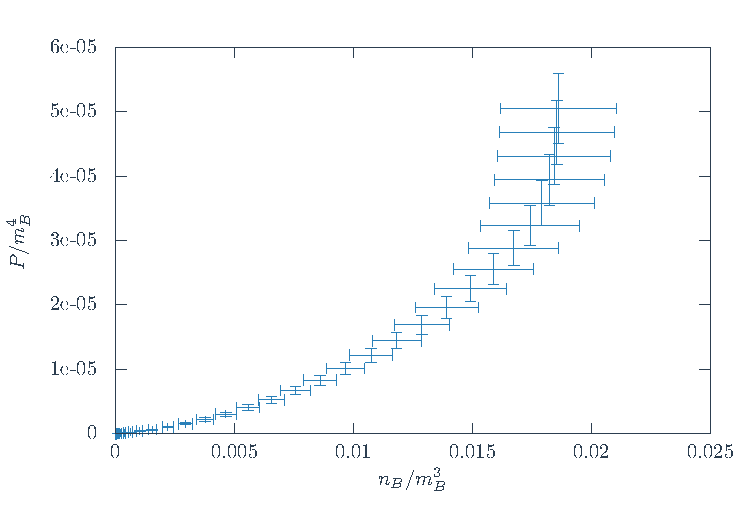
\includegraphics[width=\textwidth]{Plots/eos_cont.pdf}
  \par}
  \begin{tikzpicture}[overlay,remember picture]
    \coordinate (corner) at ([shift={(-3,2.3)}] current page.center);
    \node[anchor=north west] at (corner) [align=left,scale=0.75] {
      $T = 10$ MeV\\
      $m_{\pi} = 20$ GeV};
  \end{tikzpicture}
  }

  \note
  {
    If possible, I will try to get this plot in physical units rather than lattice units before my presentation.
  }

\end{frame}

\section{Conclusion}

\sectionframe

\begin{frame}
  \frametitle{Summary \& Outlook}

  \only<1>{
  {\color{LightUIRed} Summary}
  \begin{itemize}
    \setlength\itemsep{1em}
    \item Introduced two expansions for the lattice action
    \vspace{.5em}
      \begin{itemize}
        \setlength\itemsep{.5em}
        \item Strong coupling expansion
        \item Hopping expansion
      \end{itemize}
    \item Created a dimensionally reduced effective lattice theory
  \end{itemize}
  }

  \only<2>{
  {\color{LightUIRed} Outlook}
  \begin{itemize}
    \setlength\itemsep{1em}
    \item Look for resummations to help convergence
    \item Calculate higher order mixing terms
    \item Move more in the direction of the simulations
  \end{itemize}
  }

  \note<2>
  {
    The project with the analytic evaluations is nearing its end as we have seen both its predictive power, but also its
    limitations when studying quantities such as the nucleon binding energy (not shown, but maybe I should). Although there exists
    method for higher order evaluations of the linked cluster expansion, we are not sure if the effort will be worth it in the
    end, and might leave it as a project that can be tied into the bigger picture at a later stage. Most of the talk has of course
    focused on the effective theory and not its analytic evaluation, which we will keep pursuing.
  }
\end{frame}

\appendix
\section{Backup slides}
\sectionframe

\begin{frame}
  \frametitle{The Effective Lattice Theory}
  \framesubtitle{Mixed contributions}

  \begin{block}{Correction to $\lambda$}
    \centering
    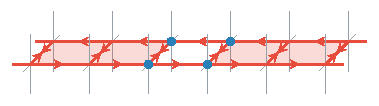
\includegraphics{Figs/lambdarenorm.pdf}
    \vspace*{-.5em}

  \begin{columns}
  \column{.35\textwidth}
  \begin{itemize}
    \item \color{LightUIBase} Rescales $\lambda$ 
  \end{itemize}
  \column{.35\textwidth}
  \begin{itemize}
    \item \color{LightUIBase} $\lambda \to \lambda(\kappa)$
  \end{itemize}
  \end{columns}
  \end{block}
  

  \begin{block}{Correction to $h_2$}
  \centering
  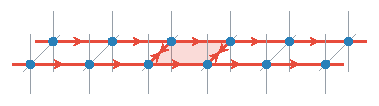
\includegraphics{Figs/h2renorm.pdf}
  \vspace*{-.5em}

  \begin{columns}
  \column{.35\textwidth}
  \begin{itemize}
    \item \color{LightUIBase} Rescales $h_2$ 
  \end{itemize}
  \column{.35\textwidth}
  \begin{itemize}
    \item \color{LightUIBase} $h_2 \to h_2(\beta)$
  \end{itemize}
  \end{columns}
  \end{block}

  \note
  {
    One can of course mix the terms from the two different expansions we are carrying out. Two examples of the possible terms can
    be seen in the figures. For these two simple cases, the mixing will only contribute as a shift in the nearest neighbour
    couplings, and can thus be absorbed by those.

    \vspace{1em}

    There are higher order mixed terms that create entierly new interactions, but those are of much higher order of what we have
    shown here.

    \vspace{1em}

    I will probably skip this slide.
  }

\end{frame}

\begin{frame}
  \frametitle{EoS in lattice units}
  {\centering%
    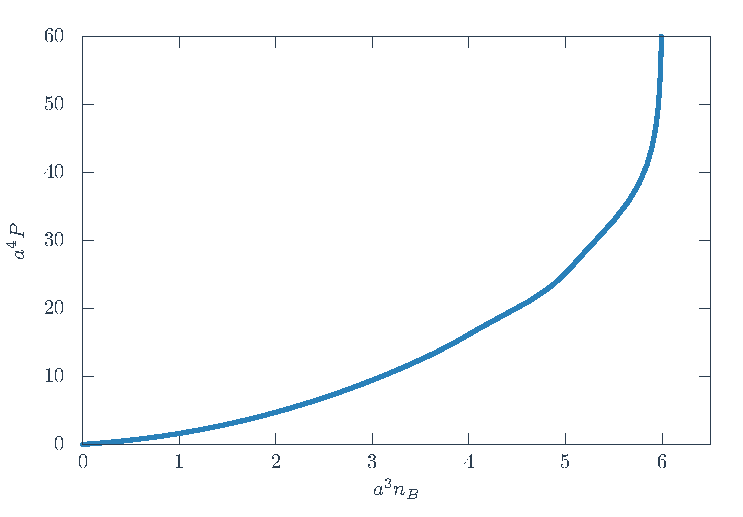
\includegraphics[width=\textwidth]{Plots/eos.pdf}
  \par}
\end{frame}

\end{document}
